\documentclass[]{article}


\usepackage{amsmath, graphicx, fullpage}

\usepackage{tikz}
\usetikzlibrary{shapes.geometric, arrows}

\tikzstyle{startstop} = [rectangle, rounded corners, minimum width=3cm, minimum height=1cm,text centered, text width=3cm, draw=black, fill=red!30]
\tikzstyle{io} = [trapezium, trapezium left angle=70, trapezium right angle=110, minimum width=3cm, minimum height=1cm, text centered, text width=2cm, draw=black, fill=blue!30]
\tikzstyle{process} = [rectangle, minimum width=3cm, minimum height=1cm, text centered, text width=3cm, draw=black, fill=orange!30]
\tikzstyle{decision} = [rectangle, minimum width=3cm, minimum height=1cm, text centered, text width=3cm, draw=black, fill=green!30]
\tikzstyle{arrow} = [thick,->,>=stealth]

\begin{document}


\title{DynoGrid\\{\Large Dynamically Load-Balanced PIC Code with an Adaptive Grid}}

\author{Scott \textsc{Luedtke}, Max \textsc{Porter}, Joel \textsc{Iventosch}, Mark \textsc{Sholte}}

\maketitle

\section{Introduction}

Particle in Cell (PIC) codes are commonly used to simulate plasma physics.  Existing codes, such as EPOCH~\cite{epoch}, allow physicists to simulate many experiments, including laser experiments.  Larger problems, such as 3D simulations of high-intensity laser experiments like those performed on the Texas Petawatt Laser (TPW), are too computationally expensive to run on modern supercomputers.  One way to bring these problems down to size is to adaptively change the grid size.  Simulations can require a very high resolution at certain sites (for example, where a laser hits a target), and orders of magnitude coarser resolution throughout the rest of the simulation.

We have developed a 3D PIC code with a standard Boris particle pusher \cite{bird}, added an adaptive grid, implemented data passing routines among nodes, and load balanced the work based on the changing grid.  Our code is not physically accurate, ommiting a field solver and ignoring many physically relevant effects, but we believe it is an accurate representation of a production code in performance characteristics and expect our load balancing to behave similarly on a production code.


\section{Code Description}
PIC codes are commonly used in computational physics.  A PIC code typically consists of an array of grid points that define electromagnetic field values, and particles that move continuously throughout the grid.  We created a fairly simple 3D laser-plasma code with externally defined fields (the laser), and physical effects such as particle collision and photon pair production omitted.  We did however add an adaptive grid which makes load balancing more complex

\subsection{Particle Pusher}
Particle-in-cell (PIC) codes used to simulate laser-plasma interactions commonly use the Boris pusher \cite{bird}, a second order accurate pusher for charged particles in electromagnetic fields.  The pusher is outlined in Fig.~\ref{fig:boris}.  Essentially, the particle is advanced a half time-step, the momentum is updated with $\vec{E}$ and rotated with $\vec{B}$, and the particle is moved a final half time-step.  With a properly set time step, a particle will never move more than one cell.


\begin{figure}[htbp]
\centering
\caption{Schematic of the Boris pusher.  The sub-cycling and current and density calculations were not implemented.}
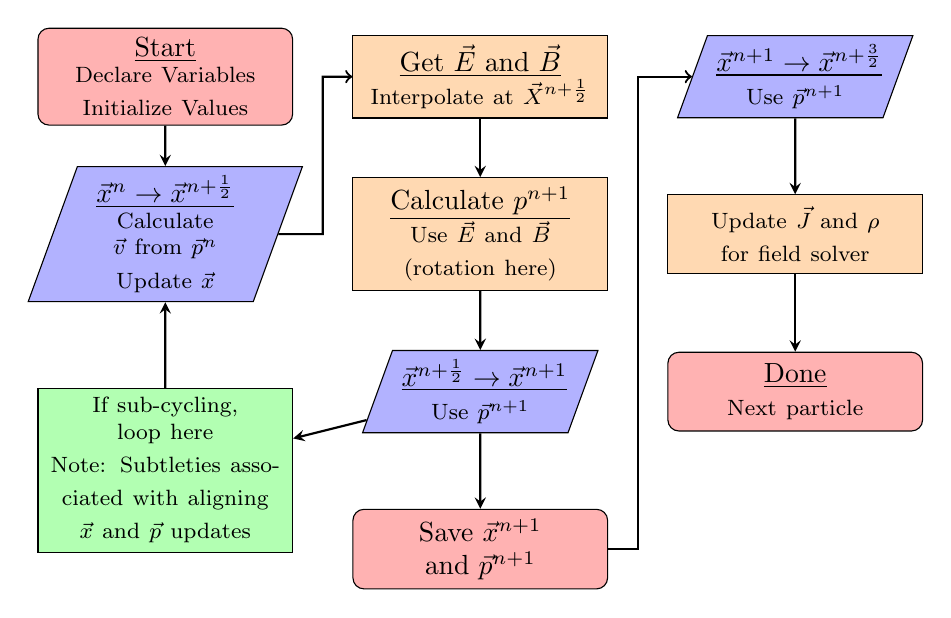
\begin{tikzpicture}[node distance=2cm]

\node (start) [startstop] {\underline{Start}\\{\footnotesize Declare Variables\\Initialize Values}};

\node(pos1)[io, below of=start]{\underline{$\vec{x}^n \rightarrow \vec{x}^{n+\frac{1}{2}}$}\\{\footnotesize Calculate $\vec{v}$ from $\vec{p}^n$\\Update $\vec{x}$}}; 

\draw[arrow](start) -- (pos1);

\node(EB)[process, right of=start, xshift=2cm]{\underline{Get $\vec{E}$ and $\vec{B}$}\\{\footnotesize Interpolate at $\vec{X}^{n+\frac{1}{2}}$}};

\draw[thick,->] (pos1) -- +(2,0) |- (EB);

\node(pn1)[process, below of=EB]{\underline{Calculate $p^{n+1}$}\\{\footnotesize Use $\vec{E}$ and $\vec{B}$ (rotation here)}};

\draw[arrow](EB) -- (pn1);

\node(pos2)[io, below of=pn1]{\underline{$\vec{x}^{n+\frac{1}{2}} \rightarrow \vec{x}^{n+1}$}\\{\footnotesize Use $\vec{p}^{n+1}$}};

\draw[arrow](pn1) -- (pos2);

\node(save)[startstop, below of=pos2]{Save $\vec{x}^{n+1}$ and $\vec{p}^{n+1}$};

\draw[arrow](pos2) -- (save);

\node(pos3)[io, right of=EB, xshift=2cm]{\underline{$\vec{x}^{n+1} \rightarrow \vec{x}^{n+\frac{3}{2}}$}\\{\footnotesize Use $\vec{p}^{n+1}$}};

\draw[thick,->] (save) -- +(2,0) |- (pos3);

\node(cur)[process, below of=pos3]{{\footnotesize Update $\vec{J}$ and $\rho$ for field solver}};

\draw[arrow](pos3) -- (cur);

\node(end)[startstop, below of=cur]{\underline{Done}\\{\footnotesize Next particle}};

\draw[arrow](cur) -- (end);

\node(sub)[decision, left of =pos2, xshift=-2cm, yshift=-1cm]{{\footnotesize If sub-cycling, loop here\\Note: Subtleties associated with aligning $\vec{x}$ and $\vec{p}$ updates}};

\draw[arrow](pos2) -- (sub);
\draw[arrow](sub) -- (pos1);

\end{tikzpicture}
\label{fig:boris}
\end{figure}

Our pusher follows the implementation in EPOCH \cite{epoch}, but with some modifications.  We use our own linear interpolation method (for simplicity), and omit the steps necessary for the field solver, which we did not implement.  We have different logic for finding the field points nearest a particle, and recursive logic to find the finest grid cell a particle is in.  In addition, we have a particle list for each base cell, and implemented logic to pass particles between lists (this makes the load balancing easier).

\subsection{Particle Lists}

\subsection{Grid Trees}

\subsection{Grid Refinement}



\section{Parallelization}

\subsection{Particle List Passer}
Particles move throughout the simulation volume and often end up in a different cell at the end of any given time step.  Since different cells can be on different processors, all processors must stop at the end of every time step to pass particles and reconcile their differences with neighbors.  To facilitate this, each base grid cell keeps a list of the particles in it and a separate list of the particles that hove moved into it.  All of the particles that need to be passed are thus in the second list of the ghost cells and there is no need to traverse a list of all particles to find those that need to be passed.  This is implemented in three steps in functions in \texttt{push.c}, \texttt{mpicomm.c}, and \texttt{mpi\_dyno.c}.

Before the communication, each processor assembles a list of its neighbors by checking the owner of each of its ghost cells.  The neighbor relationship is one-to-one, i.e., if A is B's neighbor, B is A's neighbor.  Thus each processor can communicate directly with only the processors it needs to.

First, each processor communicates to each neighbor how many particle lists it will pass, so the neighbors know how many to expect.  This is followed by an \texttt{MPI\_WaitAll} command to ensure synchronization.  Next, the neighbors communicate the size of each list to be sent, followed by another \texttt{MPI\_WaitAll}.

In the third step, the particles are themselves passed.  First, the singly-linked lists of particles are packed in to buffers that are continuous arrays of particles.  These buffers are then sent.  Memory for the receive is allocated based on the previous two communications and the receive is executed, followed by a final \texttt{MPI\_WaitAll}.  Finally, the particles are unpacked into their respective lists.

\subsection{Cell Passer}

\subsection{Load Balancer}


\section{Theoretical Performance}
For sequential performance, performance should depend on the number of particles and grid points in the simulation.  Essentially, computation time should be 
\begin{equation}
\mathcal{O}(N + M),
\end{equation}
where $N$ is the number of particles and $M$ is the number of grid points.  Since we are using an adaptive grid, $M$ is not constant, however, we will treat it as a constant here.  I (Scott) expect that full, physics-accurate simulations will refine in one area and simultaneously coarsen in another, keeping the total number (but not the processor distribution) of grid points generally constant.  This is especially true for our test problem.

\section{Performance Results}

\section{Discussion}

\section{Whodunit}
Scott Luedtke was primarily responsible for the particle pusher and load balancer.  Since this project is closely related to Scott's research, he oversaw the physics and provided general guidance for what the code should accomplish.

Max Porter worked on the grid refinement and stuff.

Joel Iventosch wrote the output and visualization routines and helped with MPI passing.  He also helped with the grid refinement.

Mark Sholte wrote much of the list functions and tree structure.  He also managed any git repository issues that arose and proved a masterful debugger.

\section{Conclusions}
























{\def\section*#1{}
\begin{thebibliography}{1}
%\footnotesize
\setlength{\itemsep}{0pt}
\bibitem{epoch}The EPOCH code was developed as part of the UK EPSRC funded projects EP/G054940/1
\bibitem{bird}Birdsall, C.K. and Langdon, A.B.  (1985). \textit{Plasma Physics via Computer Simulation}. McGraw-Hill.
%\bibitem{three}Po Kin Leung et al. 2011 Astrophysical Journal, 737 21.
%\bibitem{four}Feryal Özel et al. 2000 Astrophysical Journal, 541 234.
%\bibitem{rotation}Arefiev, Alexey V., et al. ``Temporal resolution criterion for correctly simulating relativistic electron motion in a high-intensity laser field."  Phys. Plasmas 22, 013103 (2015)

\end{thebibliography}
}




\end{document}